\section{Surface Geometry}
This section covers the basics introduced in how to represent shapes in a computer.
\subsection{Notes}
\begin{itemize}
	\item Graphics Pipeline: It refers to the sequence of steps used to create a 2D raster representation of a 3D scene. It is the process of turning a 3D model into what the computer displays. 
	\item Vertex: A point with three numbers representing its XYZ position in a plane
	\item Edge: An edge is the difference between two vertices; the segment connecting them
	\item Surface: A closed set of edges representing a face of a 3D object
	\item Polygon: A shape in space usually representing by a set of surfaces (other methods listed below)
	\item Polygon Table: A table containing a set of either vertices, edges and/or surfaces that is used to define the boundaries of a polygon. This is one method to define Polygons.
	\item Delaunay Triangulation: Given a set P of points in a plane, creates a triangular mesh DT(P) such that no point in P is inside the circumcircle of any triangle in DT(P).
\end{itemize}
   \begin{figure}[!htb]
	\center{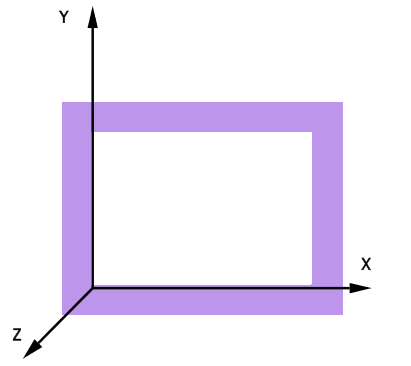
\includegraphics[width=3cm]
		{graphics/rhcoords}}
	\caption{\label{fig:rhcoords} Coordinate system assumed throughout module}
	\end{figure}
The default coordinate system assumed is right-handed: the positive x and y axes point right and up, and the negative z axis points forward. Positive rotation is counterclockwise about the axis of rotation.
\newline
Polygon Table consistency checks:
\begin{enumerate}
	\item Every vertex is listed as an endpoint of at least two edges
	\item Every surface is closed
	\item Each surface has at least one shared edge
\end{enumerate}
The order the vertices/edges are listed in a Geometric Polygon table do matter. Vertices written in clockwise order represent a surface pointing outwards. Whereas listing them counterclockwise represents an inwards pointing surface.

Meshes are a wireframe representation in which all vertices form a single set of continuous triangles, and all edges are a part of at least two triangles. Meshes can be generated by triangulation; but we covered just Delaunay Triangulation, defined above.
Meshes can also be progressive. Detail in meshes is unnecessary at farther distances, so vertices can be removed and added to create less detailed or more detailed meshes, respectively. Progress meshes do this dynamically based on viewer distance.

There are a few ways to represent polygons in a space, with boundary representations being only one method.
\begin{enumerate}
	\item Boundary Representation: Using vertices and drawing edges and surfaces from them
	\item Volumetric Models: Using simple shapes and various operations to create more complex shapes
	\item Implicit Models: Using implicit equations, such as that of a sphere, to generate shapes
	\item Parametric Models: Uses parametric equations to plot the multiple axes of a shape
\end{enumerate}
   \begin{figure}[!htb]
	\center{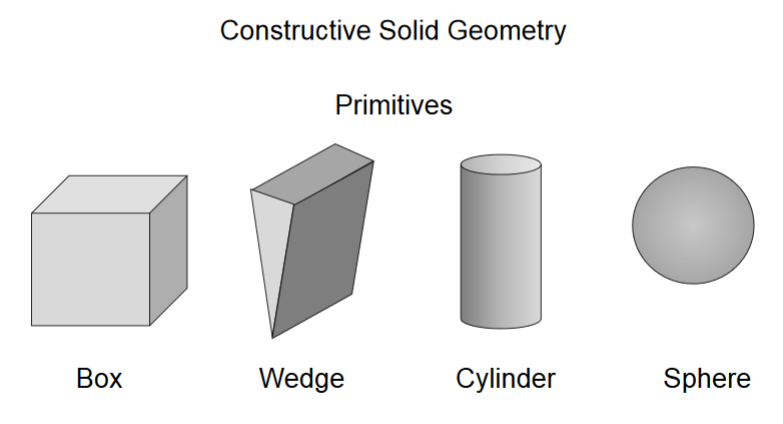
\includegraphics[width=10cm]
		{graphics/csg}}
	\caption{\label{fig:csg} Constructive Solid Geometry (CSG) Primitives}
\end{figure}
We covered a few volumetric models in the module.
\begin{enumerate}
	\item CSG: Uses primitve shapes and combines them uses set operations (union, difference, exclude, etc.) to generate new, more complex shapes.
	\item Voxels: 3D Pixels, unit cubes
	\item Octrees: Quad trees that divide in 3D space. Individual partitions are voxels
	\item Sweep: Using a 2D shape, moves that shape across a path, generating a volume in position the 2D shape occupies during its path
\end{enumerate}
One can also use implicit or parametric equations to generate shapes. Below is a list of equations that are common.
\begin{center}
	2D Circle:
	\begin{equation}
	\label{eqn:2dcirc}
	\left ( \frac{x}{r} \right )^2 + \left ( \frac{y}{r} \right )^2 = 1
	\end{equation}
	
	2D Circle - Parametric:
	\begin{equation}
	\label{eqn:2dcircpara}
	\begin{split}
	x = r\cos{\theta}  \\ y = r\sin{\theta} \\ -\pi \leq \theta \leq \pi
	\end{split}
	\end{equation}
	
	2D Ellipse - Parametric:
		\begin{equation}
	\label{eqn:2dellipsepara}
	\begin{split}
	x = r_x\cos{\theta}  \\ y = r_y\sin{\theta} \\ -\pi \leq \theta \leq \pi
	\end{split}
	\end{equation}
	
	3D Sphere:
	\begin{equation}
	\label{eqn:3dsphere}
	\left ( \frac{x}{r} \right )^2 + \left ( \frac{y}{r} \right )^2 + \left ( \frac{z}{r} \right )^2 = 1
	\end{equation}
	
	3D Ellipsoid:
	\begin{equation}
	\label{eqn:3dellipse}
	\left ( \frac{x}{r_x} \right )^2 + \left ( \frac{y}{r_y} \right )^2 + \left ( \frac{z}{r_z} \right )^2 = 1
	\end{equation}
	
	3D Sphere - Parametric:
	\begin{equation}
	\label{eqn:3dspherepara}
	\begin{split}
	x = r\cos{\phi}\cos{\theta}  \\ y = r\cos{\phi}\sin{\theta} \\ z = r\sin{\phi}\\ -\pi \leq \theta \leq \pi \\ -\pi/2 \leq \phi \leq \pi/2
	\end{split}
	\end{equation}
	
	3D Ellipsoid - Parametric:
	\begin{equation}
	\label{eqn:3dspherepara}
	\begin{split}
	x = r_x\cos{\phi}\cos{\theta}  \\ y = r_y\cos{\phi}\sin{\theta} \\ z = r_z\sin{\phi}\\ -\pi \leq \theta \leq \pi \\ -\pi/2 \leq \phi \leq \pi/2
	\end{split}
	\end{equation}
\end{center}

\subsection{Examples}
   \begin{figure}[!htb]
	\center{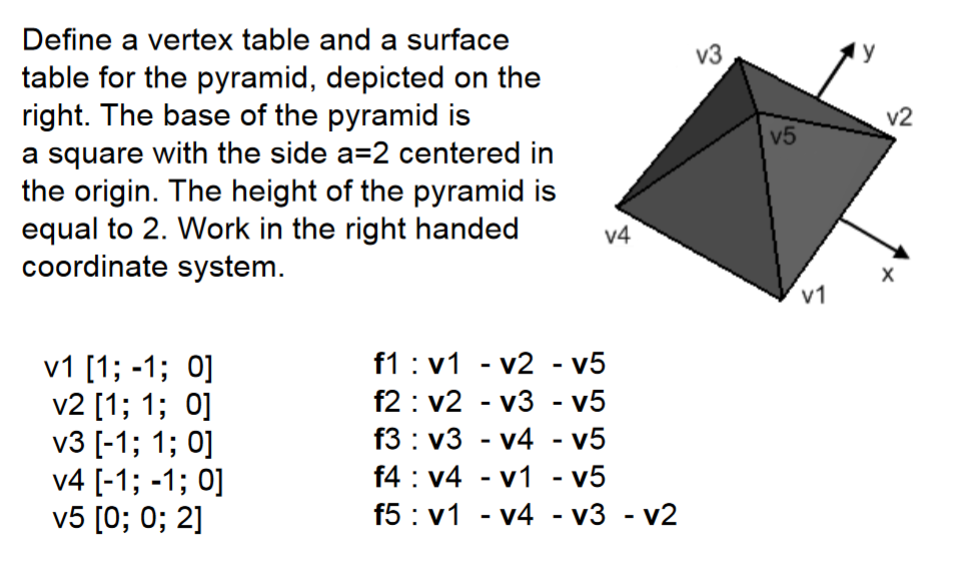
\includegraphics[width=12cm]
		{graphics/polygonTable}}
	\caption{\label{fig:pyramidPolygons} Example from Lecture}
	\end{figure}
\newpage
Further Examples are taken from quizzes and assignments
   \begin{figure}[!htb]
	\center{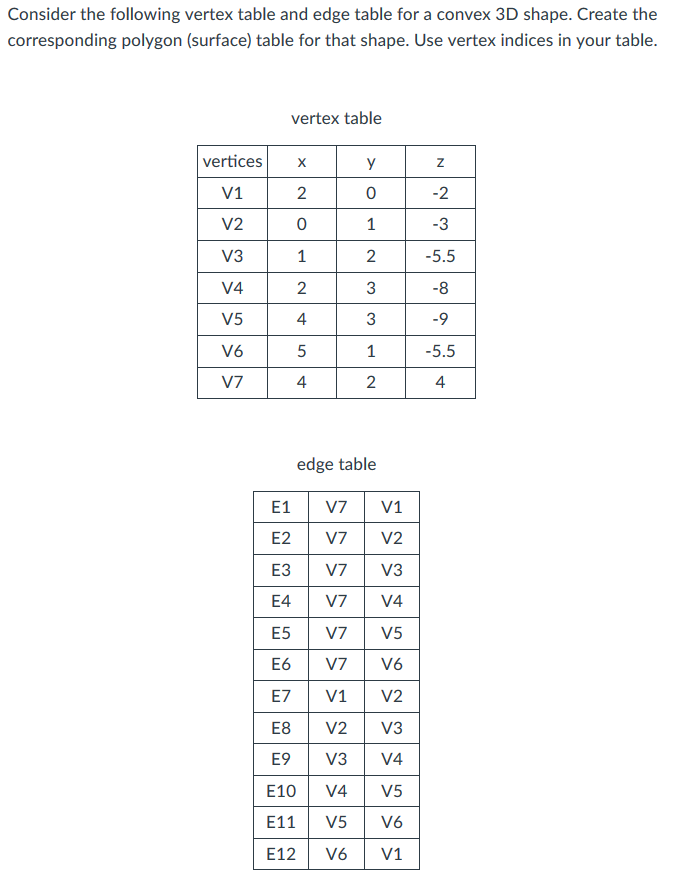
\includegraphics[width=14cm]
		{graphics/quizq1}}
	\caption{\label{fig:pyramidPolygons} Example from Quiz}
\end{figure}

Surfaces:

S1 = V1, V2, V3, V4, V5, V6

S2 = V1, V7, V2

S3 = V2, V7, V3

S4 = V2, V7, V3

S5 = V4, V7, V5

S6 = V5, V7, V6

S7 = V6, V7, V1
\subsection{Normal Vectors}
The normal vector of a surface points outwards from the surface. This is later used for lighting, projection and culling. Calculating normal vectors is a fairly simple task. For boundary polygons, the normal of a face is the cross product of two edges.
Assuming vectors A and B, the cross product is the determinant of the following matrix;

\begin{equation}
\label{eqn:crossprodMat}
\begin{bmatrix}
i & j & k\\ 
A_x & A_y & A_z\\ 
B_x & B_y & B_z
\end{bmatrix}
\end{equation}

Which can be minimized to the following (longer) equation;

\begin{equation}
\label{eqn:crossprodLine}
N = \begin{bmatrix}
A_yB_z - A_zB_y\\ 
A_zB_x - A_xB_z\\ 
A_xB_y - A_yB_x
\end{bmatrix}
\end{equation}

To know which vectors to use for A and B, simply select an edge on a surface, and you use your right hand with your thumb pointing outwards and curl your hand around in the direction until the first vector hits your hand. Alternatively, you can piece it together by looking at the figure.
  \begin{figure}[!htb]
	\center{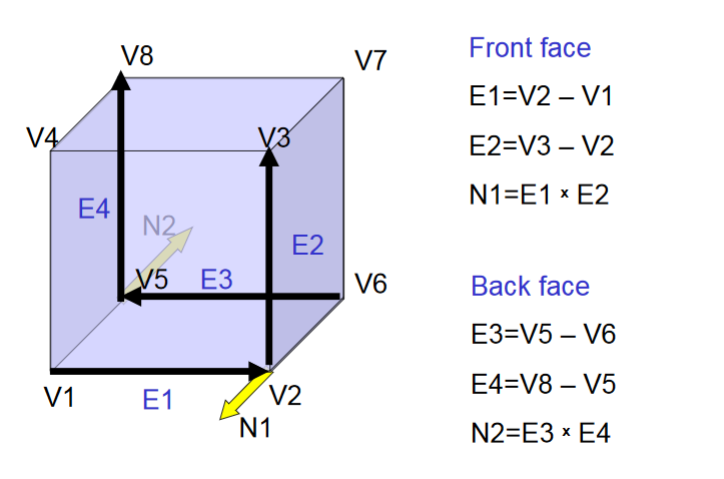
\includegraphics[width=10cm]
		{graphics/normal}}
	\caption{\label{fig:normalCube} Normal Vector of cube from lecture}
\end{figure}

\subsection{Further Sources}
	\href{https://www.tutorialspoint.com/computer_graphics/computer_graphics_surfaces.htm}{Surface Representations}
	\newline
	\href{https://www.cs.cmu.edu/afs/cs/academic/class/15462-s09/www/lec/04/lec04.pdf}{Alternate Lecture}
\newpage
\section{Transforms}
This section covers simple transformation matrices.
\subsection{Notes}
\begin{itemize}
	\item Transformation: a function that can be applied to each of the points in a geometric object to produce a new object.
	\item Translation: A geometric transform that adds a given translation amount to each coordinate of a point. Translation is used to move objects without changing their size or orientation.
	\item Rotation: A geometric transform that rotates each point by a specified angle about some point (in 2D) or axis (in 3D).
	\item Scaling: A geometric transform that multiplies each coordinate of a point by a number called the scaling factor. Scaling increases or decreases the size of an object, but also moves its points closer to or farther from the origin.
\end{itemize}
Transformations are applied to geometric objects to move them around. This is valuable when considering camera positions, or when laying out a world in a video game.
Transformations can be applied as equations for each dimensions eg. \[T_x = x + t_x\] is the new x-position when applying the translation. However, there is a lack of uniformity between different transforms, some requiring x and y more than once, others being matrices. To standardize transforms, we instead use \textit{Homogeneous Transformation Matrices}. Convert a 2D point to a 3D point by setting z = 1, and apply the transforms as matrices by replacing the variable found in each matrix template. This is an easy way of standardizing the equations, and allows for easy transforms by multiplying the transformations together before multiplying them with the point.

For example, applying a Translation {T} and then a Rotation {R} can be done by multiplying {RT} first and then multiplying the new transform matrix with the original points. This also makes it more efficient to move more than one point when they share the same transform, as it only need one multiplication per-point rather than one per-transform per-point.
\subsection{Transformation Matrices}

\begin{equation}
\label{eqn:crossprodLine}
T_{2D} = \begin{bmatrix}
1 & 0 & T_x\\ 
0 & 1 & T_y\\ 
0 & 0 & 1\\ 
\end{bmatrix}
\end{equation}

\begin{equation}
\label{eqn:crossprodLine}
S_{2D} = \begin{bmatrix}
S_x & 0 & 0\\ 
0 & S_y & 0\\ 
0 & 0 & 1\\ 
\end{bmatrix}
\end{equation}

\begin{equation}
\label{eqn:crossprodLine}
R_{2D} = \begin{bmatrix}
\cos{\theta} & -\sin{\theta} & T_x\\ 
\sin{\theta} & \cos{\theta} & T_y\\ 
0 & 0 & 1\\ 
\end{bmatrix}
\end{equation}

\begin{equation}
\label{eqn:crossprodLine}
T_{3D} =\begin{bmatrix}
1 & 0 & 0 & T_x\\ 
0 & 1 & 0 & T_y\\ 
0 & 0 & 1 & T_z\\
0 & 0 & 0 & 1 
\end{bmatrix}
\end{equation}

\begin{equation}
\label{eqn:crossprodLine}
S_{3D} = \begin{bmatrix}
S_x & 0 & 0 & 0\\ 
0 & S_y & 0 & 0\\ 
0 & 0 & S_z & 0\\
0 & 0 & 0 & 1 
\end{bmatrix}
\end{equation}

\begin{equation}
\label{eqn:crossprodLine}
R_{3D_X} = \begin{bmatrix}
1 & 0 & 0 & 0\\ 
0 & \cos{\theta} & -\sin{\theta} & 0\\ 
0 & \sin{\theta} & \cos{\theta} & 0\\
0 & 0 & 0 & 1 
\end{bmatrix}
\end{equation}

\begin{equation}
\label{eqn:crossprodLine}
R_{3D_Y} = \begin{bmatrix}
\cos{\theta} & 0 & \sin{\theta} & 0\\ 
0 & 1 & 0 & 0\\ 
-\sin{\theta} & 0 & \cos{\theta} & 0\\
0 & 0 & 0 & 1 
\end{bmatrix}
\end{equation}

\begin{equation}
\label{eqn:crossprodLine}
R_{3D_Z} = \begin{bmatrix}
\cos{\theta} & -\sin{\theta} & 0 & 0\\ 
\sin{\theta} & \cos{\theta} & 0 & 0\\ 
0 & 0 & 1 & 0\\
0 & 0 & 0 & 1
\end{bmatrix}
\end{equation}
\subsection{Examples}

\subsection{References}
\href{http://math.hws.edu/graphicsbook/c2/s3.html}{Quick Overview}

\newpage
\section{Lighting}
This section covers things related to lighting and shading of objects in a scene.
\subsection{Notes}
\begin{itemize}
	\item Diffuse: Non-shiny illumination
	\item Specular: Shiny reflections
	\item Ambient: background illumination
\end{itemize}
\textbf{Ambient Light}
\begin{itemize}
	\item Global background light
	\item No direction
	\item Does not depend on anything
\end{itemize}
\textbf{Diffuse Light}
\begin{itemize}
	\item Parallel Light Rays originating from a source direction
	\item Contributes to Diffuse and Specular Term
\end{itemize}
\textbf{Spot Light}
\begin{itemize}
	\item Originates from a single source point
	\item Conic dispersion of light, intensity is a function of distance
	\item More realistic
\end{itemize}
\textbf{Surface Properties}
\begin{itemize}
	\item Geometry - Position, orientation
	\item Colour - reflectance and Absorption spectrum
	\item Micro-structure - defines reflectance properties
\end{itemize}
\textbf{Shading Models}
\begin{itemize}
	\item	Flat shading is the simplest shading model. Each rendered polygon has a single normal vector; shading for the entire polygon is constant across the surface of the polygon. With a small polygon count, this gives curved surfaces a faceted look.
	
	\item	Phong shading is the most sophisticated of the three. Each rendered polygon has one normal vector per vertex; shading is performed by interpolating the vectors across the surface and computing the color for each point of interest.
	
	\item	Gouraud shading is in between the two: like Phong shading, each polygon has one normal vector per vertex, but instead of interpolating the vectors, the color of each vertex is computed and then interpolated across the surface of the polygon.
\end{itemize}
  \begin{figure}[!htb]
	\center{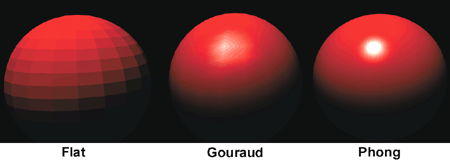
\includegraphics[width=10cm]
		{graphics/shadingModels}}
	\caption{\label{fig:normalCube} Shading Model Differences}
\end{figure}
\subsection{Phong Shading Equation}
\begin{equation}
\label{eqn:phongEqn}
\begin{split}
Colour = Ambient + Diffuse + Specular \\
Colour = I_aK_a + I_dK_d\cos{\theta_L} + I_sK_s\cos^n{\theta_S} 
\end{split}
\end{equation}

\textbf{Ambient Term}
This is very easy. It is the $K_{a}$ term multiplied with the Ambient intensity $I_{a}$.
\begin{equation}
\label{eqn:phongAmbient}
Ambient = I_aK_a
\end{equation}

\textbf{Diffuse Term}
The diffuse term is usually straight forward.. It is the $K_{d}$ term multiplied with the Light source intensity $I_{d}$. The angle $\theta$ between the light source and the normal of the surface is then computed, and the $cos(\theta)$ is multiplied to obtain the full term.
\begin{equation}
\label{eqn:phongDiffuse}
Diffuse =  I_dK_d\cos{\theta_L}
\end{equation}

\begin{figure}[!htb]
\center{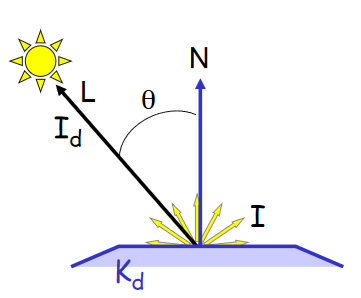
\includegraphics[width=5cm]
	{graphics/diffuse}}
\caption{\label{fig:diffuse} Diffuse term overview}
\end{figure}

\textbf{Specular Term}
The specular term needs a few more steps. It is the $K_{s}$ term multiplied with the reflected Light source intensity $I_{s}$. This is the ray that is bounced off of the surface, and is $\theta_L$ away from the normal of the surface. This intensity is multiplied by the $\cos$ of the angle $\theta_S$, the angle between the reflected ray and the line of sight from the camera. The $\cos$ is raised to the $n_{th}$ power, a factor known as a shininess factor that is usually given.

\begin{equation}
\label{eqn:phongSpecular}
Diffuse =  I_dK_d\cos^n{\theta_S}
\end{equation}
\begin{figure}[!htb]
	\center{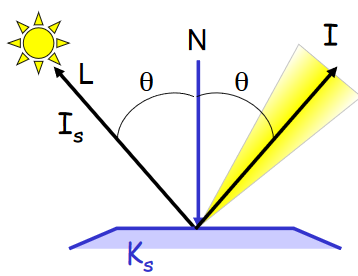
\includegraphics[width=5cm]
		{graphics/specular}}
	\caption{\label{fig:specular} Specular term overview}
\end{figure}

\subsection{Examples}

\newpage
\section{Projection}
\newpage
\section{Texture Mapping}
\newpage
\section{Past Exam Practice}